% !TEX root = quickstep.tex
\chapter{Design and Implementation of Quickstep System}\label{chap:quickstep}

\section{Introduction}
Query processing systems today face a host of challenges that were not as prominent just a few years ago. 
A key change has been dramatic changes in the hardware landscape that is driven by the need to consider energy as a first-class (hardware) design parameter. Across the entire processor-IO hierarchy, the hardware paradigm today looks very different than it did just a few years ago. Consequently, we are now experiencing a growing \textit{deficit} (illustrated in Figure~\ref{fig-deficit}) between the pace of hardware performance improvements and the pace that is demanded of data processing kernels to keep up with the growth in data volumes.

Our attempt to pay off this deficit is through a system called \Quickstep.
Our goal is to exploit the full (parallel) processing power that is locked in commodity multi-core servers today.
We describe the initial version of Quickstep that targets single-node in-memory read-mostly analytic workloads.
Quickstep uses mechanisms that allow for \textit{high intra-operator parallelism}. 
Such mechanisms are critical to exploit the full potential of the high level of hardware compute parallelism that is present in modern servers (the dotted orange line in Figure~\ref{fig-deficit}).

Unlike most research database management systems (DBMSs), \Quickstep\ has a storage manager with a block layout, where each block behaves like a mini self-contained database~\cite{ChasseurP13}.
This ``independent'' block-based storage design is leveraged by a highly parallelizable query execution paradigm in which independent \textit{work orders} are generated at the block level. Query execution then amounts to creating and scheduling work orders, which can be done in a generic way. Thus, the scheduler is a crucial system component, and the Quickstep scheduler cleanly separates scheduling policies from the underlying scheduling mechanisms. This separation allows the system to elastically scale the resources that are allocated to queries, and to adjust the resource allocations dynamically to meet various policy-related goals.

Recognizing that random memory access patterns and materialization costs often dominate the execution time in main-memory DBMSs, Quickstep uses a number of query processing techniques that take the ``drop early, drop fast'' approach: eliminating redundant rows as early as possible, as fast as possible. For instance, Quickstep aggressively pushes down complex disjunctive predicates involving multiple tables using a %novel
predicate over-approximation scheme. Quickstep also uses cache-efficient filter data structures to pass information across primary key-foreign key equijoins,  eliminating semi-joins entirely in some cases. 

\begin{figure}
	\centering
	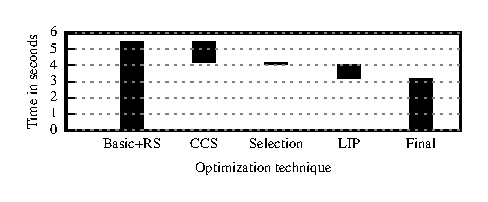
\includegraphics[width=0.75\textwidth]{system/figures/tpch-q10-waterfall.pdf}
	\caption{\textbf{A waterfall chart showing the impact of various techniques in Quickstep for query 10 from the TPC-H benchmark running on a 100 scale factor database. RS (Row Store), and CCS (Compressed Column Store) are both supported in Quickstep (see Section~\ref{block-structure}). Basic and Selection are template metaprogramming optimizations (described in Section~\ref{vectorization}), which relate to the efficiency of predicate and expression evaluation. LIP (Lookahead Information Passing, described in Section~\ref{sec:lip}) is a technique to improve join performance. Starting with a configuration (Basic + RS), each technique is introduced one at a time to show the individual impact of each technique on this query.}}
	\label{fig:tpch-q10-waterfall}
\end{figure}

Overall, the key contributions of our work are as follows:\\

\textbf{Cohesive collection of techniques:} We present the first end-to-end design for Quickstep. This system brings together in a single artifact a number of mechanisms for in-memory query processing such as support for multiple storage formats, a template metaprogramming approach to both manage the software complexity associated with supporting multiple storage formats and to evaluate expressions on data in each storage format efficiently, and novel query optimization techniques.
The impact of each mechanism depends on the workload, and our system brings these mechanisms together as a whole.
For example, the waterfall chart in Figure~\ref{fig:tpch-q10-waterfall} shows the contributions of various techniques on the performance of TPC-H Query 10.

\paragraph{Novel query processing techniques:} We present Quickstep's use of techniques to aggressively push down complex disjunctive predicates involving multiple relations, as well as to eliminate certain types of equijoins using \textit{exact filters}.

\paragraph{Manageability:} The design of the system focuses on ease-of-use, paying attention to a number of issues, including employing methods such as using a holistic approach to memory management, and elastically scaling query resource usage at runtime to gracefully deal with concurrent queries with varying query priorities.

\paragraph{Comparison with other systems:} We also conduct an end-to-end evaluation comparing \Quickstep\ with a number of other systems. These system are: Spark~\cite{Spark, SparkSQL}, PostgreSQL~\cite{postgres}, MonetDB~\cite{monetdb}, and VectorWise~\cite{vectorwise}. Our results show that in many cases, Quickstep is faster by an order-of-magnitude, or more.

We also leverage the multiple different storage implementations in Quickstep to better understand the end-to-end impact of the popular row store and column store methods on the SSB and TPC-H queries. To the best of our knowkedge, an apples-to-apples comparison of these benchmark queries does not exist. We show that overall column stores are still preferred, though the speed up overall is only about 2X. Earlier comparisions, e.g.~\cite{AbadiMH08}, have been indirect comparisons of this aspect of storage management for the SSB benchmark across two different systems, and show far larger (6X) improvements. %We also find that overall for the SSB benchmark compression does not produce significant benefits.

\paragraph{Open source:} Quickstep\ is available as open-source, which we hope helps the reproducability goal that is being pursued in our community~\cite{BonnetMBCGGHIIJKKMOPRTYFS11, ManegoldMAFGHHKKLLORSSWS09, ManolescuAADMPSSZS08}. It also allows other researchers to use this system as a platform when working on  problems where the impact of specific techniques can be best studied within the context of the overall system behavior.

The remainder of this chapter is organized as follows: The overall Quickstep architecture is presented in the next section. The storage manager in presented in Section~\ref{storage-manager}. The query execution and scheduling methods are presented in Sections~\ref{query-exec} and~\ref{sec:query-opt} respectively. Empirical results are presented in Section~\ref{evaluation}, and related work is presented in Section~\ref{related}. Finally, Section~\ref{conclusions} contains our concluding remarks.